\section{Arrays and Lists}
\begin{itemize}
    \item As you know arrays have a fixed list, once it is declared of a certain size it stays that size unless you reallocate it to an array of a bigger size. But keep in mind that this is inefficient and the initial estimate might require more and more space.
\end{itemize}

%%%%%%%%%%%%%%%%%%%%%%%%%%%%%%%%%%%%%%%%%%%%%%%%%%%%%%
\section{What is a linked list?}
\begin{itemize}
    \item An array in memory is like an array of cells:
        \begin{figure}[H]
            \centering
            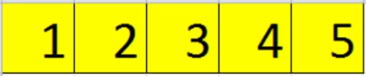
\includegraphics[width=\width\textwidth]{./figs/20221027220708.png}
            %\caption{}
        \end{figure}
    
    \item With a linked list we do not allocate in a contigous chunk but rather on an element by element bases.
        \begin{figure}[H]
            \centering
            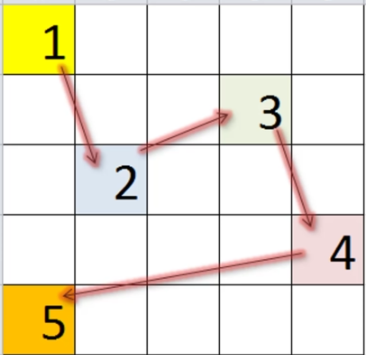
\includegraphics[width=\width\textwidth]{./figs/20221027220746.png}
            %\caption{}
        \end{figure}
    
    \item What allowes us to do this is pointers, because as I require an extra item, the location of the item is likely to be anywhere, not next to it. Thus I need to use pointers, and iterating a linked list uses pointers too. Each element of the list holds a pointer to the next element, if there is no next element then it will hold a null pointer.
\end{itemize}

%%%%%%%%%%%%%%%%%%%%%%%%%%%%%%%%%%%%%%%%%%%%%%%%%%%%%%
\section{Singly linked list}
\begin{itemize}
    \item Here is an example of a linked list of integers:
        \begin{minted}[autogobble]{c}
            #include <stdio.h>
            #include <stdlib.h>
            #include <string.h>

            typedef struct listitem {
                struct listitem *next;
                int data;
            } LISTITEM;

            int main() {
                LISTITEM *listhead, *temp;
                listhead = NULL;

                for (int i = 0; i < 3; i++) {
                    temp = malloc(sizeof(LISTITEM));
                    temp->data = i;
                    temp->next = listhead;
                    listhead = temp;
                }

                temp = listhead;
                while (temp != NULL) {
                    printf("list item: current is %p; next is %p; data is %d\n", temp, temp->next, temp->data);
                    temp = temp->next;
                }
                return 0;
            }
        \end{minted}
    
    \item In the following code what it looks like in memory is like this:
        \begin{figure}[H]
            \centering
            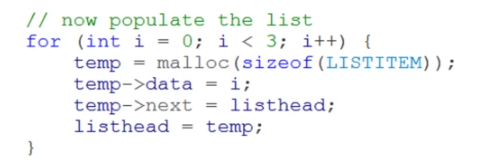
\includegraphics[width=\width\textwidth]{./figs/20221027221603.png}
            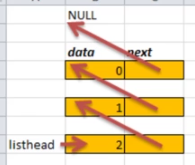
\includegraphics[width=\width\textwidth]{./figs/20221027221645.png}
            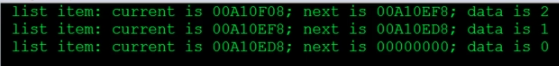
\includegraphics[width=\width\textwidth]{./figs/20221027221655.png}
            %\caption{}
        \end{figure}
    
    \item In this example the new element is added in the begining of the list, you can add them at the end too, this is trivial for our purposes. Usually it is more efficient to add new elements to a start of a list.
\end{itemize}

%%%%%%%%%%%%%%%%%%%%%%%%%%%%%%%%%%%%%%%%%%%%%%%%%%%%%%
\section{To free or not to free?}
\begin{itemize}
    \item the free function needs to be called everytime we use malloc. But if the allocated memory is used through out all of the lifetime of the program we don't need to do that, that is if the memory remains referenced by pointers (through out all of the lifetime of the program) and remain in use the operating system will deallocate it after. (*This is actually not mentioned here but what happens is the OS will whipe the code page of the heap program in memory, thus we don't need to free it, but if we were to no longer need the memory we need to free it.)
\end{itemize}

%%%%%%%%%%%%%%%%%%%%%%%%%%%%%%%%%%%%%%%%%%%%%%%%%%%%%%
\section{Doubly linked lists}
\begin{itemize}
    \item In a singly linked list each element holds the address of the next element, but we can only move from the begining to the right and not back, sometimes it is useful to be able to move to the left too. A doubly linked list is a list which holds an address to the next element and to the previous element.
        \begin{figure}[H]
            \centering
            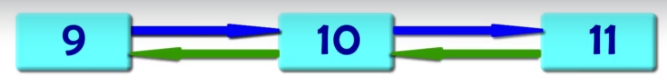
\includegraphics[width=\width\textwidth]{./figs/20221027222341.png}
            %\caption{}
        \end{figure}
\end{itemize}

%%%%%%%%%%%%%%%%%%%%%%%%%%%%%%%%%%%%%%%%%%%%%%%%%%%%%%
\section{Programming a doubly-linked List}
\begin{itemize}
    \item See the following code to get the doubly linked list.
        \begin{minted}[autogobble]{c}
            #include <stdio.h>
            #include <stdlib.h>
            #include <string.h>
            typedef struct listitem {
                struct listitem *next;
                struct listitem *prev;
                int data;
            } LISTITEM;
            int main() {
                LISTITEM head, *temp;

                head.next = (LISTITEM*)&head;
                head.prev = (LISTITEM*)&head;
                head.data = -1;
                
                for (int i = 0; i < 3; i++) {
                    temp = malloc(sizeof(LISTITEM));
                    temp->data = i;
                    temp->next = head.next;
                    head.next = temp;
                    temp->prev = &head;
                    temp->next->prev = temp;
                }
                return 0;
            }
        \end{minted}
\end{itemize}

%%%%%%%%%%%%%%%%%%%%%%%%%%%%%%%%%%%%%%%%%%%%%%%%%%%%%%
\section{Initializing a doubly-linked list}
\begin{itemize}
    \item Initializing a doubly linked list is not as straight forward as initializing. With a doubly linked list the pointers are both ways. When adding the first element the first element by definition does not have a previous element nor a next. We will add NULL pointers and when the next is added we will change.
\end{itemize}
